\PassOptionsToPackage{unicode=true}{hyperref} % options for packages loaded elsewhere
\PassOptionsToPackage{hyphens}{url}
%
\documentclass[ignorenonframetext,aspectratio=169,]{beamer}
\setbeamertemplate{caption}[numbered]
\setbeamertemplate{caption label separator}{: }
\setbeamercolor{caption name}{fg=normal text.fg}
\beamertemplatenavigationsymbolsempty
\usepackage{lmodern}
\usepackage{amssymb,amsmath}
\usepackage{ifxetex,ifluatex}
\usepackage{fixltx2e} % provides \textsubscript
\ifnum 0\ifxetex 1\fi\ifluatex 1\fi=0 % if pdftex
  \usepackage[T1]{fontenc}
  \usepackage[utf8]{inputenc}
  \usepackage{textcomp} % provides euro and other symbols
\else % if luatex or xelatex
  \usepackage{unicode-math}
  \defaultfontfeatures{Ligatures=TeX,Scale=MatchLowercase}
\fi
\usetheme[]{shadow}
% use upquote if available, for straight quotes in verbatim environments
\IfFileExists{upquote.sty}{\usepackage{upquote}}{}
% use microtype if available
\IfFileExists{microtype.sty}{%
\usepackage[]{microtype}
\UseMicrotypeSet[protrusion]{basicmath} % disable protrusion for tt fonts
}{}
\IfFileExists{parskip.sty}{%
\usepackage{parskip}
}{% else
\setlength{\parindent}{0pt}
\setlength{\parskip}{6pt plus 2pt minus 1pt}
}
\usepackage{hyperref}
\hypersetup{
            pdftitle={Bespoke bioinformatic modeling},
            pdfauthor={A. Grant Schissler},
            pdfborder={0 0 0},
            breaklinks=true}
\urlstyle{same}  % don't use monospace font for urls
\newif\ifbibliography
% Prevent slide breaks in the middle of a paragraph:
\widowpenalties 1 10000
\raggedbottom
\setbeamertemplate{part page}{
\centering
\begin{beamercolorbox}[sep=16pt,center]{part title}
  \usebeamerfont{part title}\insertpart\par
\end{beamercolorbox}
}
\setbeamertemplate{section page}{
\centering
\begin{beamercolorbox}[sep=12pt,center]{part title}
  \usebeamerfont{section title}\insertsection\par
\end{beamercolorbox}
}
\setbeamertemplate{subsection page}{
\centering
\begin{beamercolorbox}[sep=8pt,center]{part title}
  \usebeamerfont{subsection title}\insertsubsection\par
\end{beamercolorbox}
}
\AtBeginPart{
  \frame{\partpage}
}
\AtBeginSection{
  \ifbibliography
  \else
    \frame{\sectionpage}
  \fi
}
\AtBeginSubsection{
  \frame{\subsectionpage}
}
\setlength{\emergencystretch}{3em}  % prevent overfull lines
\providecommand{\tightlist}{%
  \setlength{\itemsep}{0pt}\setlength{\parskip}{0pt}}
\setcounter{secnumdepth}{0}

% set default figure placement to htbp
\makeatletter
\def\fps@figure{htbp}
\makeatother


\title{Bespoke bioinformatic modeling}
\author{A. Grant Schissler}
\providecommand{\institute}[1]{}
\institute{Department of Mathematics and Statistics University of Nevada, Reno}
\date{}

\begin{document}
\frame{\titlepage}

\begin{frame}{%
\protect\hypertarget{science-through-interdiscplinary-efforts}{%
Science through interdiscplinary efforts}}

\begin{itemize}
\tightlist
\item
  Progress in many fields of scientific inquiry require experts from
  various fields: biology, chemistry, computer science, genetics,
  medicine, mathematics/statistics, etc.
\item
  Bioinformatics is a prime example of such a field, with interest and
  expertise across domains .
\item
  When I was invited to speak here, Dr.~Wallace said that many of you
  all are dealing with ’omics data and was curious what bioinformatic
  expertise is available on campus.
\item
  So I’ll share my thoughts on this and discuss 2 relevant biomedical
  gene expression projects.
\end{itemize}

\end{frame}

\begin{frame}{%
\protect\hypertarget{special-considerations-for-bioinformatics}{%
Special considerations for bioinformatics}}

\begin{itemize}
\tightlist
\item
  There are many standard tools and pipelines to measure high-throughput
  ’omics data (such as RNA-sequencing, mass spectrometry, microarray,
  etc).
\item
  There are also many choices available for the downstream analysis —
  differentially expressed genes DEGs, pathway enrichment, etc.
\item
  Keeping up with the advanced tools is a job in itself. We at UNR are
  lucky to have a bioinformatics core to run experiments, quantify
  (measure), process (noise correction, etc), and perform statistical
  analyses.
\item
  If you have standard research question and experimental design, it is
  best to talk to them early and work together through the process. And
  enjoy the high quality data!
\end{itemize}

\end{frame}

\begin{frame}{%
\protect\hypertarget{what-to-do-when-conventional-methods-fail}{%
What to do when conventional methods fail?}}

\begin{itemize}
\tightlist
\item
  But sometimes you’d like to understand data from nonstandard setups.
\item
  For example, are your sample sizes inherently limited? Such as rare
  diseases / species.
\item
  And sometimes you aren’t sure how to conduct statistical
  inferences\ldots{}
\end{itemize}

\end{frame}

\begin{frame}{%
\protect\hypertarget{so-you-result-to-looking-at-charts-like-this}{%
So you result to looking at charts like this}}

\begin{columns}
\begin{column}{0.5\textwidth}  
    \begin{center}
    \begin{itemize}
        \item Most developed in early 20th century, fragile, eclipsed by more recent tools
        \item Often users don’t know they are using models
        \item Symptom of naive adhearance to science through falisfication
    \end{itemize}
     \end{center}
\end{column}
\begin{column}{0.5\textwidth}
    \includegraphics[height=0.9\paperheight, keepaspectratio]{../Stan_talk_neurolecture_series/stats_flow_chart_v2014.pdf}
\end{column}
\end{columns}

\end{frame}

\begin{frame}{%
\protect\hypertarget{that-is-a-good-time-to-talk-to-an-applied-statistician}{%
That is a good time to talk to an applied statistician}}

\begin{itemize}
\tightlist
\item
  When you are in this situation someone like me is a good collaborator.
\item
  Discussions should begin early, not after getting the data and trying
  to recover.
\item
  But most statisticians can’t resist seeing data at any point, so it is
  worth a shot.
\item
  Now I’ll discuss 2 bioinformatic projects that resulting produced
  novel methods in challenging/nonstandard settings.
\end{itemize}

\end{frame}

\begin{frame}{%
\protect\hypertarget{project-1-n1pas}{%
Project 1 N1PAS}}

\begin{itemize}
\tightlist
\item
  Do alternatively spliced genes in tumor aggregate into biological
  pathways?
\item
  Does this signal inform on cancer survival?
\item
  Can this be discovered in a single-subject experimental design (nof1)?
\item
  You need a tailored (bespoke) method to handle this question.
\item
  This lead to the development of N-of-1-\emph{pathways} Alternatively
  Spliced (N1PAS).
\end{itemize}

\end{frame}

\begin{frame}{%
\protect\hypertarget{n1pas-the-general-idea}{%
N1PAS The general idea}}

\begin{itemize}
\item We'd like a methodology to estimate complex biological dysregulation using paired samples from cancer patients.
\item This dysregulation relates to coordinated differential protein isoform usage within biological pathways.
\item But we seek a single-subject framework for precision medicine.
\item Moreover, the setting involves large-scale simultaneous signification under correlated test statistics.
  \item This is extremely challenging when you only can analyze one patient's data at a time.
\end{itemize}

\end{frame}

\begin{frame}{%
\protect\hypertarget{rna-seq-isoform-counts-from-lung-cancer-tumors}{%
RNA-seq isoform counts from lung cancer tumors}}

\begin{table}
\label{tab:TNBCdata}
\begin{tabular}{c|l|ccc}
\hline
$i$ & Gene symbol & Isoform ID & Normal & Tumor \\
\hline
1 &  \emph{DDX11L1}   & uc011lsn.1  & 0   & 0 \\
2 &  \emph{DDX11L9}     & uc010unu.1  & 2   & 23 \\
3 &  \emph{DDX11L1}    & uc010uoa.1  & 0   & 0 \\
4 &  \emph{OR4F5}   & uc002bgz.2  & 8   & 16 \\
5 &  \emph{DQ597235}     & uc002bic.2  & 0   & 0 \\
6 &  \emph{DQ599768}    & uc010zzl.1  & 115 &   159 \\
$\vdots$ &   $\vdots$       & $\vdots$ & $\vdots$ & $\vdots$  \\
73599 &  \emph{abParts}  & uc011nby.1  & 0   & 0  \\
\hline
\end{tabular}
\end{table}
\addtocounter{footnote}{1}\footnotetext{The Cancer Genome Atlas (TGCA) LUSC data set}

\end{frame}

\begin{frame}{%
\protect\hypertarget{alternatively-spliced-genes-asgs-in-a-few-pictures}{%
Alternatively spliced genes (ASGs) in a few pictures}}

\begin{figure}[htb]
   \centering
 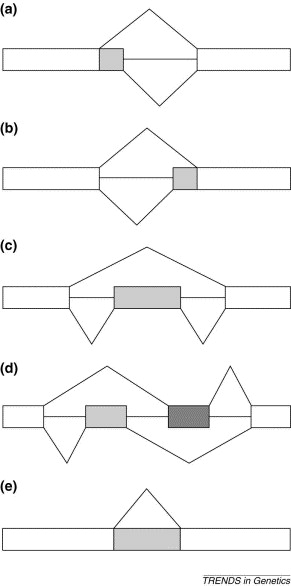
\includegraphics[keepaspectratio,width=\textwidth,height=0.75\textheight]{../n1pas/figures/splice_figure.jpg}
    \end{figure}
    \note{enormous diversity possible (some genes code for 10s of 1000s mRNAs}

Graveley (2001)

\end{frame}

\begin{frame}{%
\protect\hypertarget{gene-set-analysis-in-biomedical-research}{%
Gene set analysis in biomedical research}}

Gene set analyses Khatri, Sirota, and Butte (2012) give mechanistic
interpretation by aggregating gene-level results. Widely-used
method:\textasciitilde{}GSEA Subramanian et al. (2005). Example
ontology:\textasciitilde{}KEGG Kanehisa and Goto (2000).

\begin{block}{Kyoto encyclopedia of genes and genomes (KEGG)}

\begin{table}
         \begin{tabular}{lll}
           ID & Description & Gene\\
           \hline
           hsa00010 & Glycolysis Gluconeogenesis & LDHAL6B\\
           hsa00010 & Glycolysis Gluconeogenesis & ADH1B\\
           $\vdots$ & $\vdots$ & $\vdots$\\
           hsa05416 & Viral myocarditis & MYH8\\
         \end{tabular}
\end{table}

\end{block}

\end{frame}

\begin{frame}{%
\protect\hypertarget{the-n-of-1-pathways-framework}{%
The N-of-1-\emph{pathways} framework}}

\begin{figure}[htb]
    \centering
\includegraphics[keepaspectratio,width=\textwidth,height=0.6\textheight]{../n1pas/figures/N-of-1-pathways-dep-flowchart.pdf}
\end{figure}

\end{frame}

\begin{frame}{%
\protect\hypertarget{correlation-and-large-scale-simultaneous-sign.testing}{%
Correlation and Large-Scale Simultaneous Sign.\textasciitilde{}Testing}}

\begin{figure}[htb]
  \centering
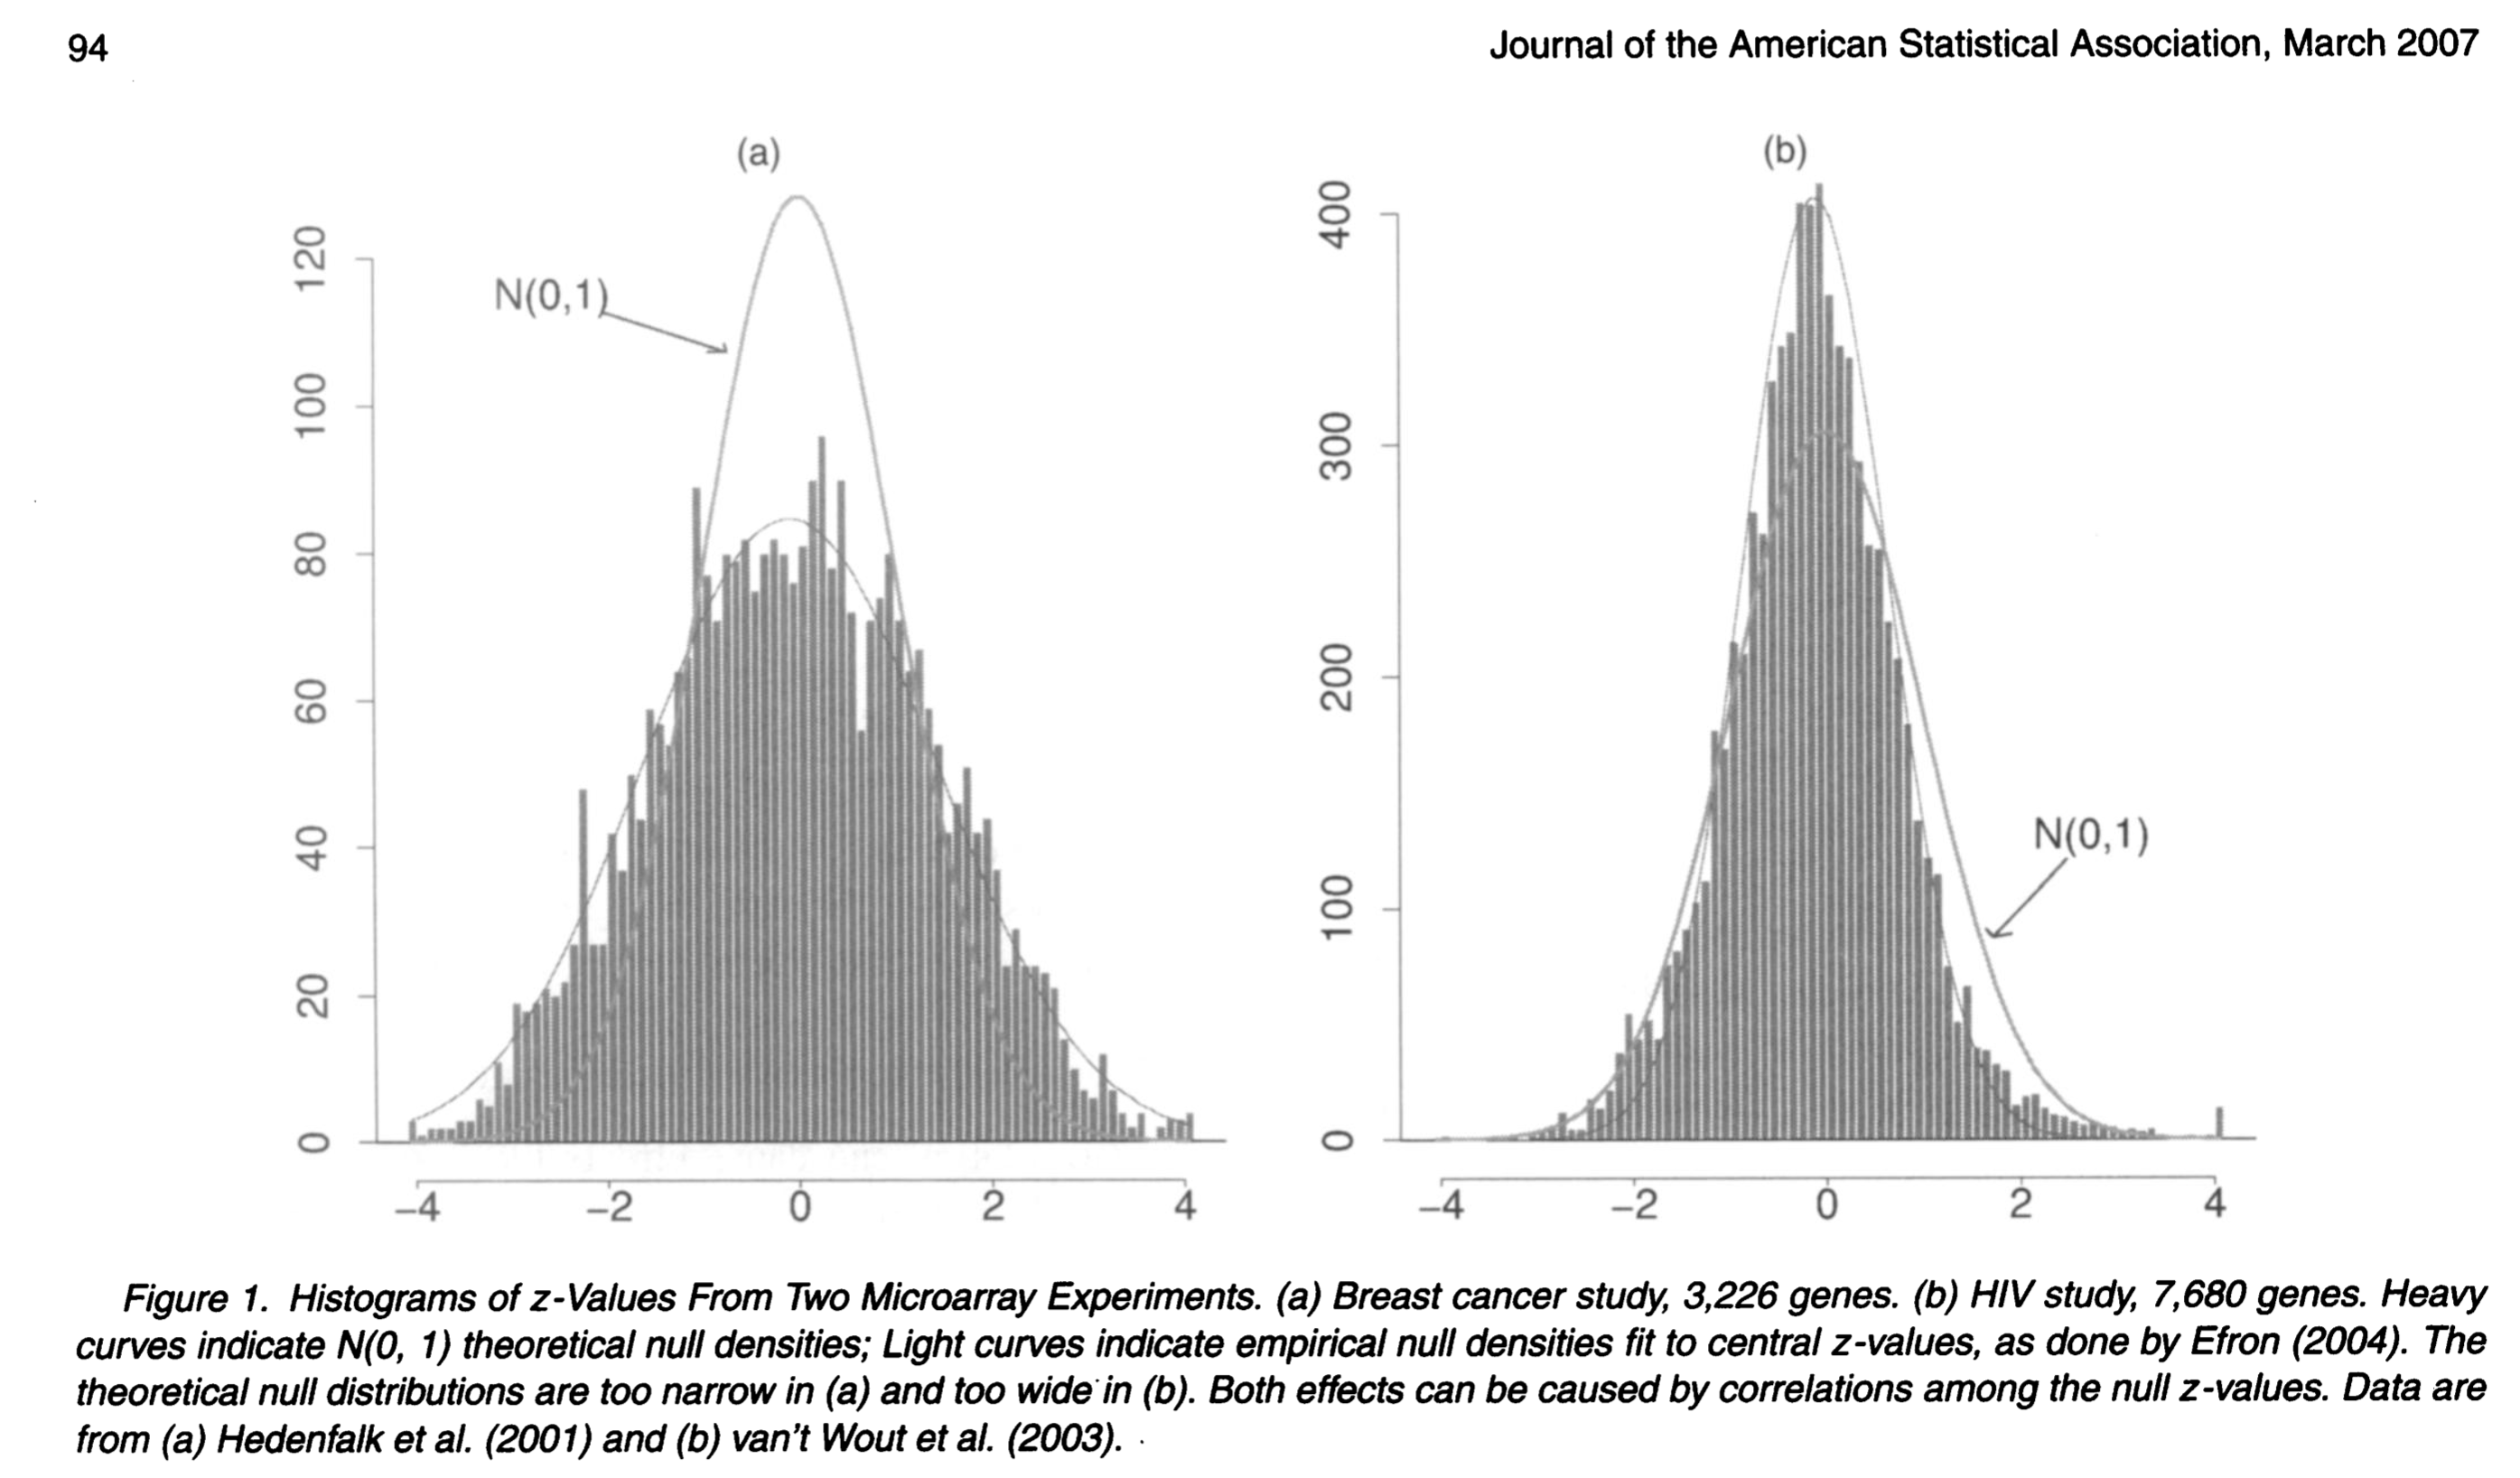
\includegraphics[keepaspectratio,width=\textwidth,height=0.75\textheight]{../n1pas/figures/Efron2007_figure1.png}
   \end{figure}

Efron (2007)

\end{frame}

\begin{frame}{%
\protect\hypertarget{efrons-local-false-discovery-rate}{%
Efron’s local false discovery rate}}

Assume that \(N\) values can be sorted into two classes (‘null’ and
‘nonnull’), occurring with probabilities of \(p_{0}\) or
\(p_{1}=1-p_{0}\), \begin{align*}
     p_{0} & = Pr\{null\} & f_{0}(z), if \; null \\
     p_{1} & = Pr\{nonnull\} & f_{1}(z), if \; nonnull
   \end{align*} Define the \emph{null subdensity} as
\(f^{+}_{0}=p_{0}f_{0}(z)\) and the \emph{mixture density} as
\(f(z)=p_{0}f_{0}(z) + p_{1}f_{1}(z)\). Then define the local false
discovery rate (locFDR) as the Bayesian posterior probability that a
case is null given \(z\),

\begin{equation*}
fdr(z) = Pr\{null | z \} = \frac{p_{0}f_{0}(z)}{f(z)}= f^{+}_{0}/f(z).
     \end{equation*} Efron (2013)

\end{frame}

\begin{frame}{%
\protect\hypertarget{quantification-of-differential-alternative-splicing}{%
Quantification of differential alternative splicing}}

We follow Johnson \& Purdom and use of the Hellinger distance to
quantify alternative splicing between a pair of samples. Let the
estimates of isoform expression for a sample \(A\) be denoted as
\(x_{gA1},\ldots,x_{gAK_{g}}\) for the \(K_{g}\) distinct isoforms
annotated to gene \(g\). We define the relative isoform usage as the
vector of relative proportions of each isoform,
\(p_{gA}= \left( \frac{x_{gA1}}{\sum_{k=1}^{K_{g}} x_{gAk}}, \ldots, \frac{x_{gAK_{g}}}{\sum_{k=1}^{K_{g}} x_{gAk}} \right)\)

Then define the Hellinger distance \begin{equation*}
H_{g}(p_{gA}, p_{gB}) = 1 / \sqrt{2} \sum_{k=1}^{K_{g}} \left( \sqrt{ \frac{x_{gAk}}{\sum_{k=1}^{K_{g}} x_{gAk}}  }  - \sqrt{ \frac{x_{gBk}}{\sum_{k=1}^{K_{g}} x_{gBk}} } \right)^{2}
    \end{equation*} Johnson and Purdom (2017)

\end{frame}

\begin{frame}{%
\protect\hypertarget{n-of-1-pathways-alternatively-spliced-n1pas}{%
N-of-1-pathways Alternatively Spliced (N1PAS)}}

\begin{figure}[htb]
  \centering 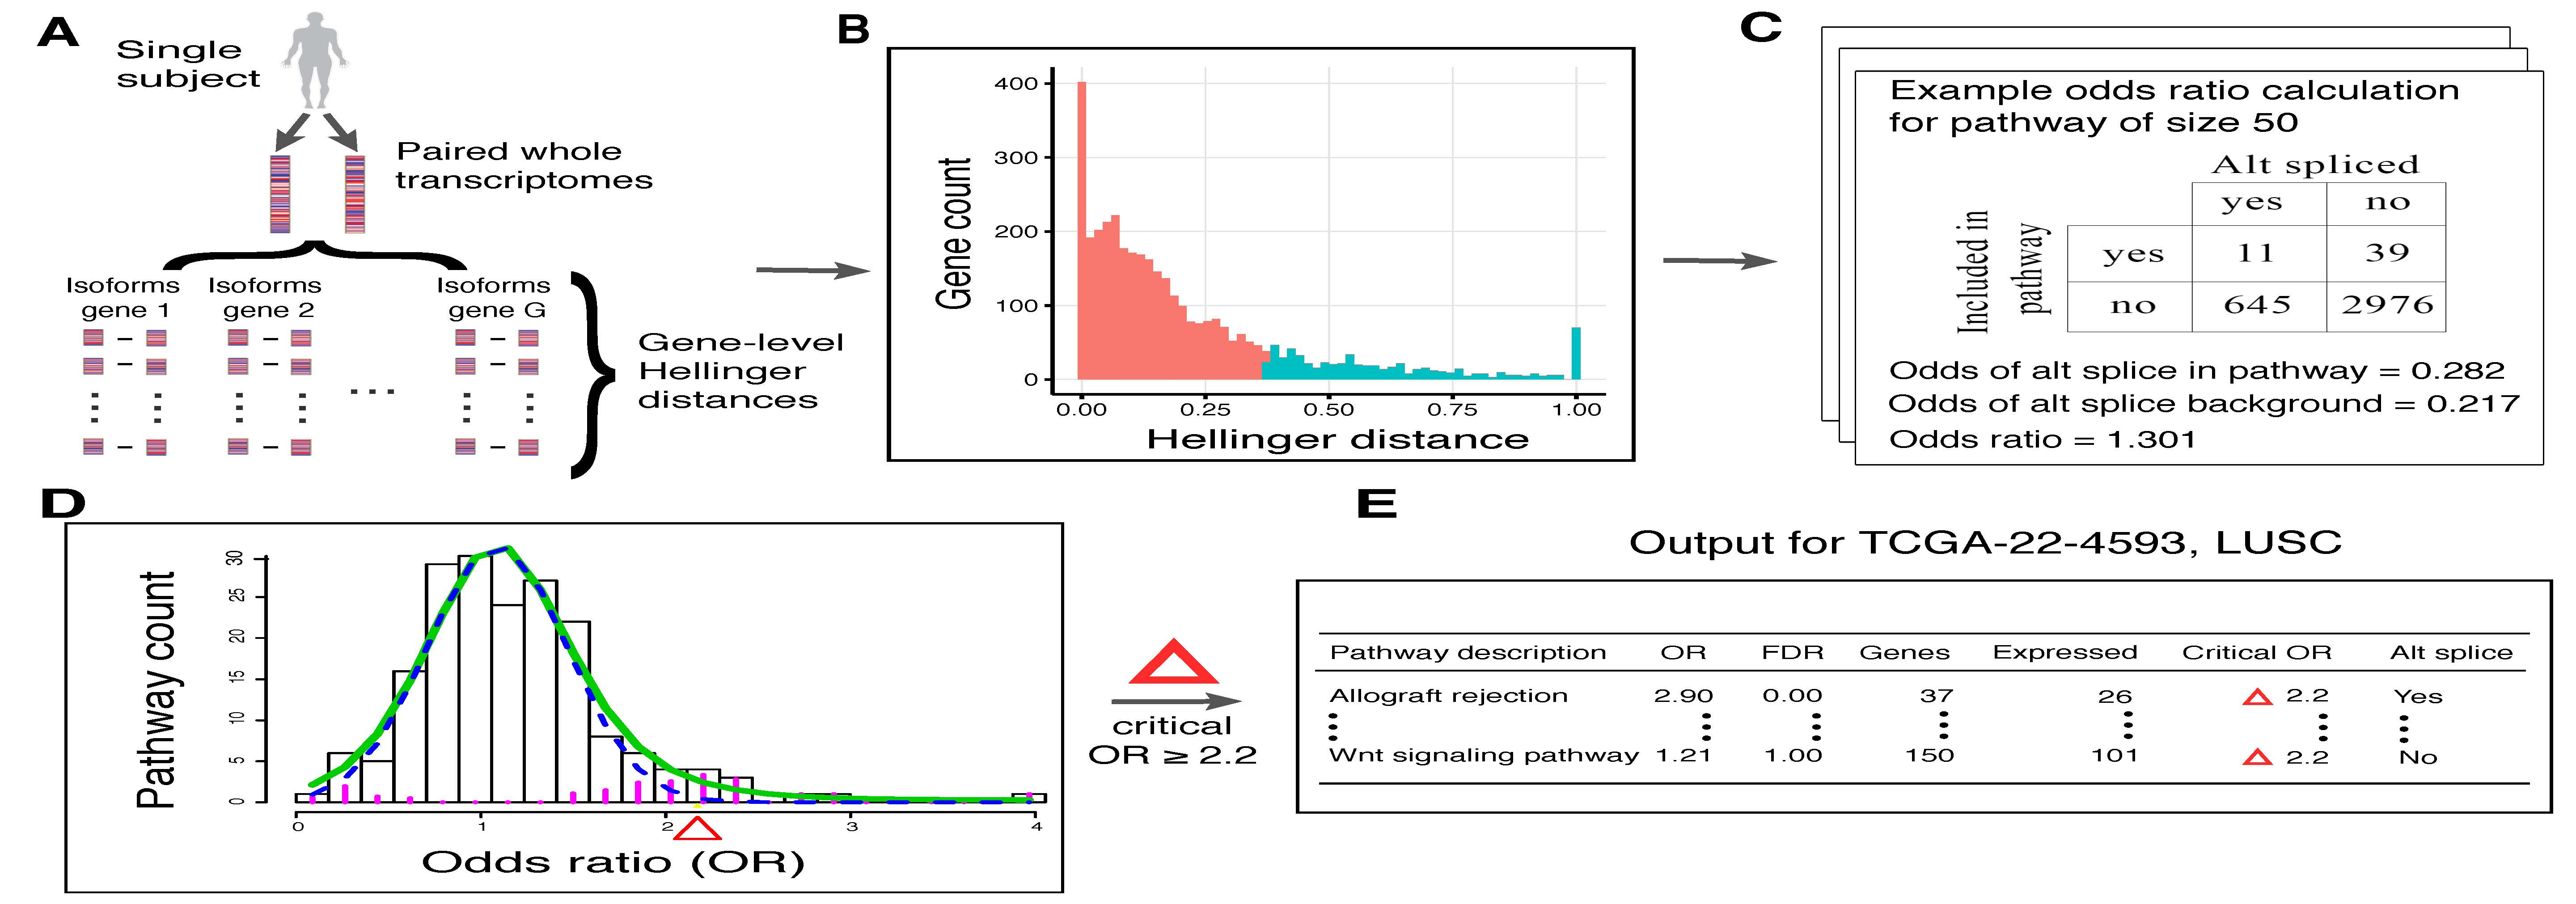
\includegraphics[keepaspectratio,width=\textwidth,height=0.8\textheight]{../n1pas/figures/Figure1.jpg}
\end{figure}

\end{frame}

\begin{frame}{%
\protect\hypertarget{tcga-data-sets-to-guide-development}{%
TCGA data sets to guide development}}

\begin{figure}[htb]
  \centering 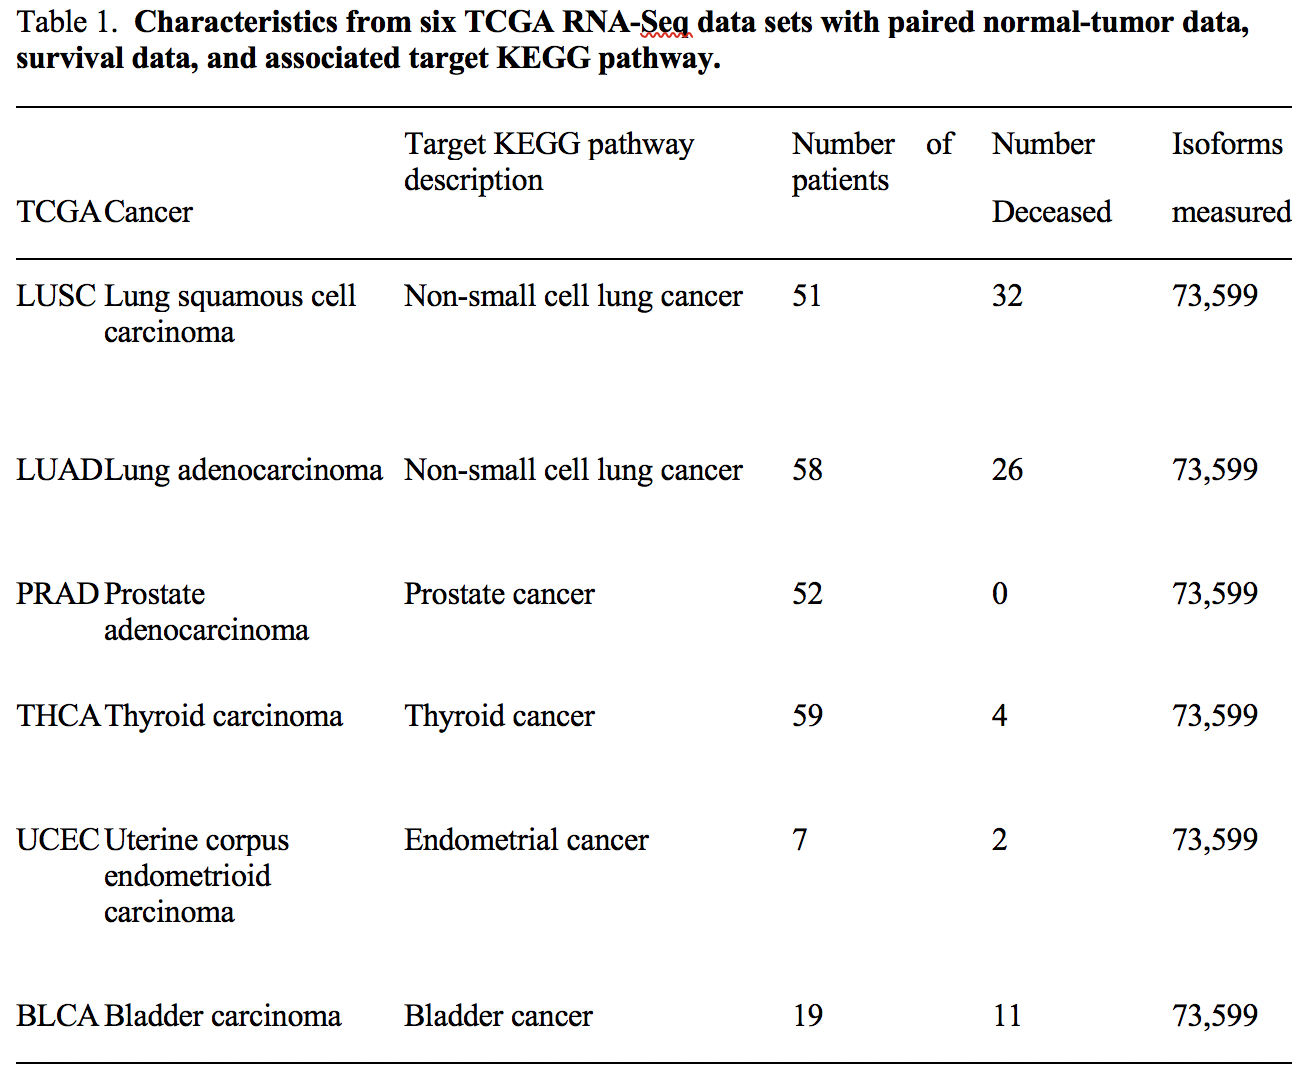
\includegraphics[keepaspectratio,width=\textwidth,height=0.8\textheight]{../n1pas/figures/datasets.png}
\end{figure}

\end{frame}

\begin{frame}{%
\protect\hypertarget{monte-carlo-evaluation}{%
Monte Carlo evaluation}}

\begin{itemize}
  \item Trying the simulate parameterically is challenging as the isoform counts are ultra high-dimensional, multivariate, and discrete
  \item Instead we chose to permute in a subject-specific way:~find the distribution of Hellinger distances for the 4133 genes annotated to KEGG pathways. Then permute gene labels to create null distribution of pathway odds ratios.
    \item The effect size corresponds to the proportion of ASGs within a pathway $\pi$, relative to the subject-specific background level of ASGs ($\pi_{all}$).
  \end{itemize}

\end{frame}

\begin{frame}{%
\protect\hypertarget{simulation-settings-and-procedure}{%
Simulation settings and procedure}}

\begin{itemize}
  \item 6 TCGA data sets explored, for a total of 246 patients.
    \item For each patient, compute Hellinger distances for each gene and use 2-means to cluster into ASG or not classes.
    \item Let $G=\{15, 30, 50, 100\}$ be the number of expressed genes in the specified pathway. Select at random a KEGG pathway with this number of genes.
    \item Let the effect size $\pi=\{0, 0.05, 0.10, 0.15, 0.20\}$.
    \item Select $G \times (\pi + \pi_{all})$ genes within the specified pathway at random to be from the ASG class and the remaining pathway genes from the non-ASG class.
    \item Apply N1PAS 100 times and determine empirical power as detection rate of the specified pathway.
      \item This results in 246 * 5 effect sizes * 4 pathway size * 100 reps = 492,000 simulated N1PAS runs.
\end{itemize}

\end{frame}

\begin{frame}{%
\protect\hypertarget{permutation-based-simulated-false-discovery-rates}{%
Permutation-based simulated false discovery rates}}

\begin{figure}[htb]
  \centering \includegraphics[keepaspectratio,width=\textwidth,height=0.8\textheight]{../n1pas/figures/Figure6noGeneSetSize_gs.pdf}
\end{figure}

\end{frame}

\begin{frame}{%
\protect\hypertarget{permutation-based-simulated-power}{%
Permutation-based simulated power}}

\begin{figure}[htb]
  \centering 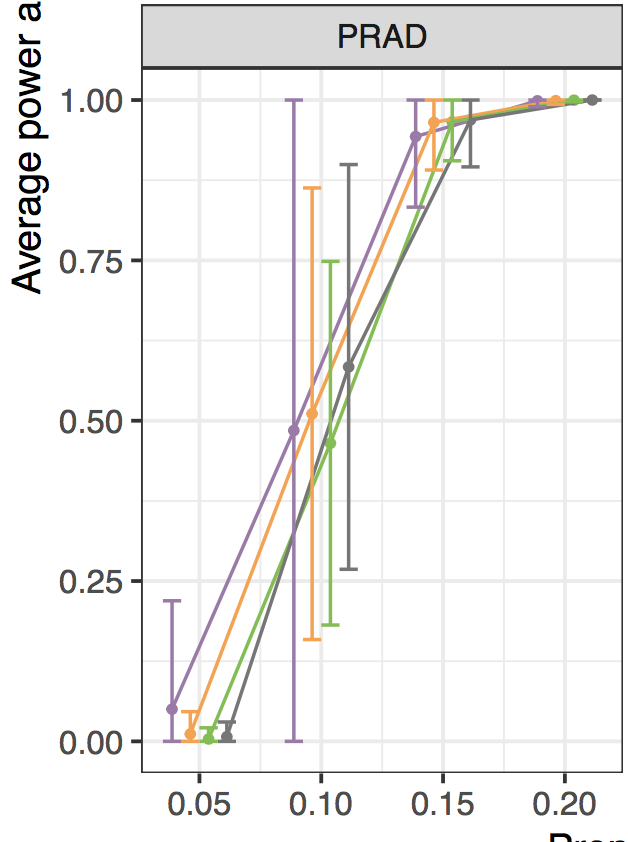
\includegraphics[keepaspectratio,width=\textwidth,height=0.9\textheight]{../n1pas/figures/Figure7_one.png}
\end{figure}

\textbackslash{}end\{frame\}

\end{frame}

\begin{frame}{%
\protect\hypertarget{permutation-based-simulated-power-1}{%
Permutation-based simulated power}}

\begin{figure}[htb]
  \centering \includegraphics[keepaspectratio,width=\textwidth,height=0.9\textheight]{../n1pas/figures/Figure7.pdf}
\end{figure}

\end{frame}

\begin{frame}{%
\protect\hypertarget{kegg-validation-study-results}{%
KEGG validation study results}}

\begin{figure}[htb]
  \centering 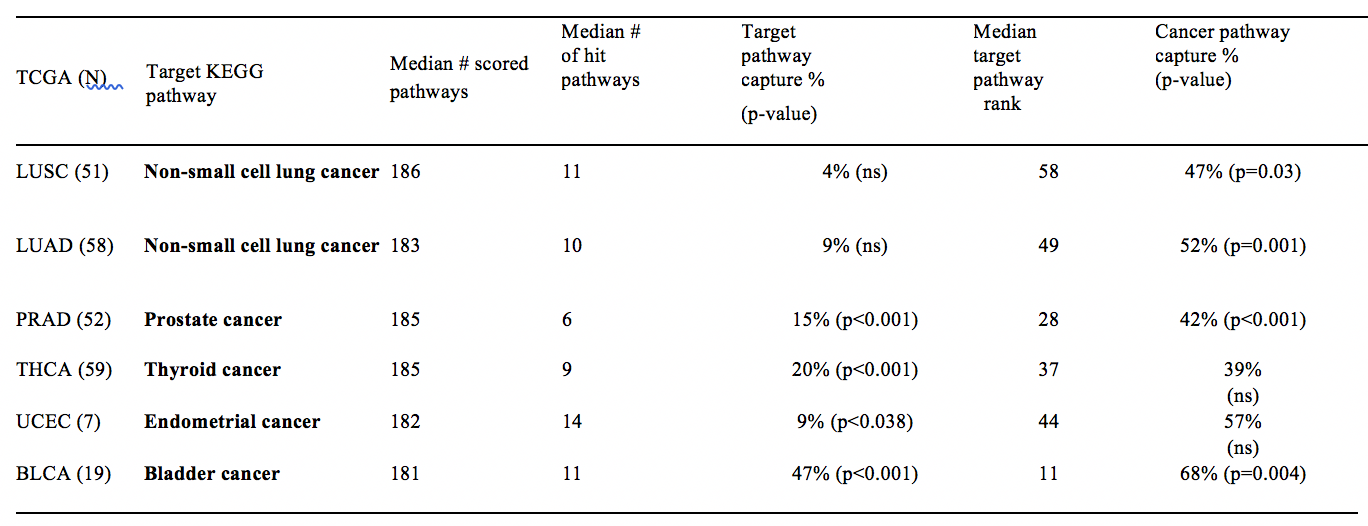
\includegraphics[keepaspectratio,width=\textwidth,height=0.8\textheight]{../n1pas/figures/table2.png}
\end{figure}

\end{frame}

\begin{frame}{%
\protect\hypertarget{boxplots-of-patient-specific-odds-ratios-or-of-the-target-kegg-pathway-for-the-six-tcga-data-sets}{%
Boxplots of patient-specific odds ratios (OR) of the target KEGG pathway
for the six TCGA data sets}}

\begin{figure}[htb]
  \centering 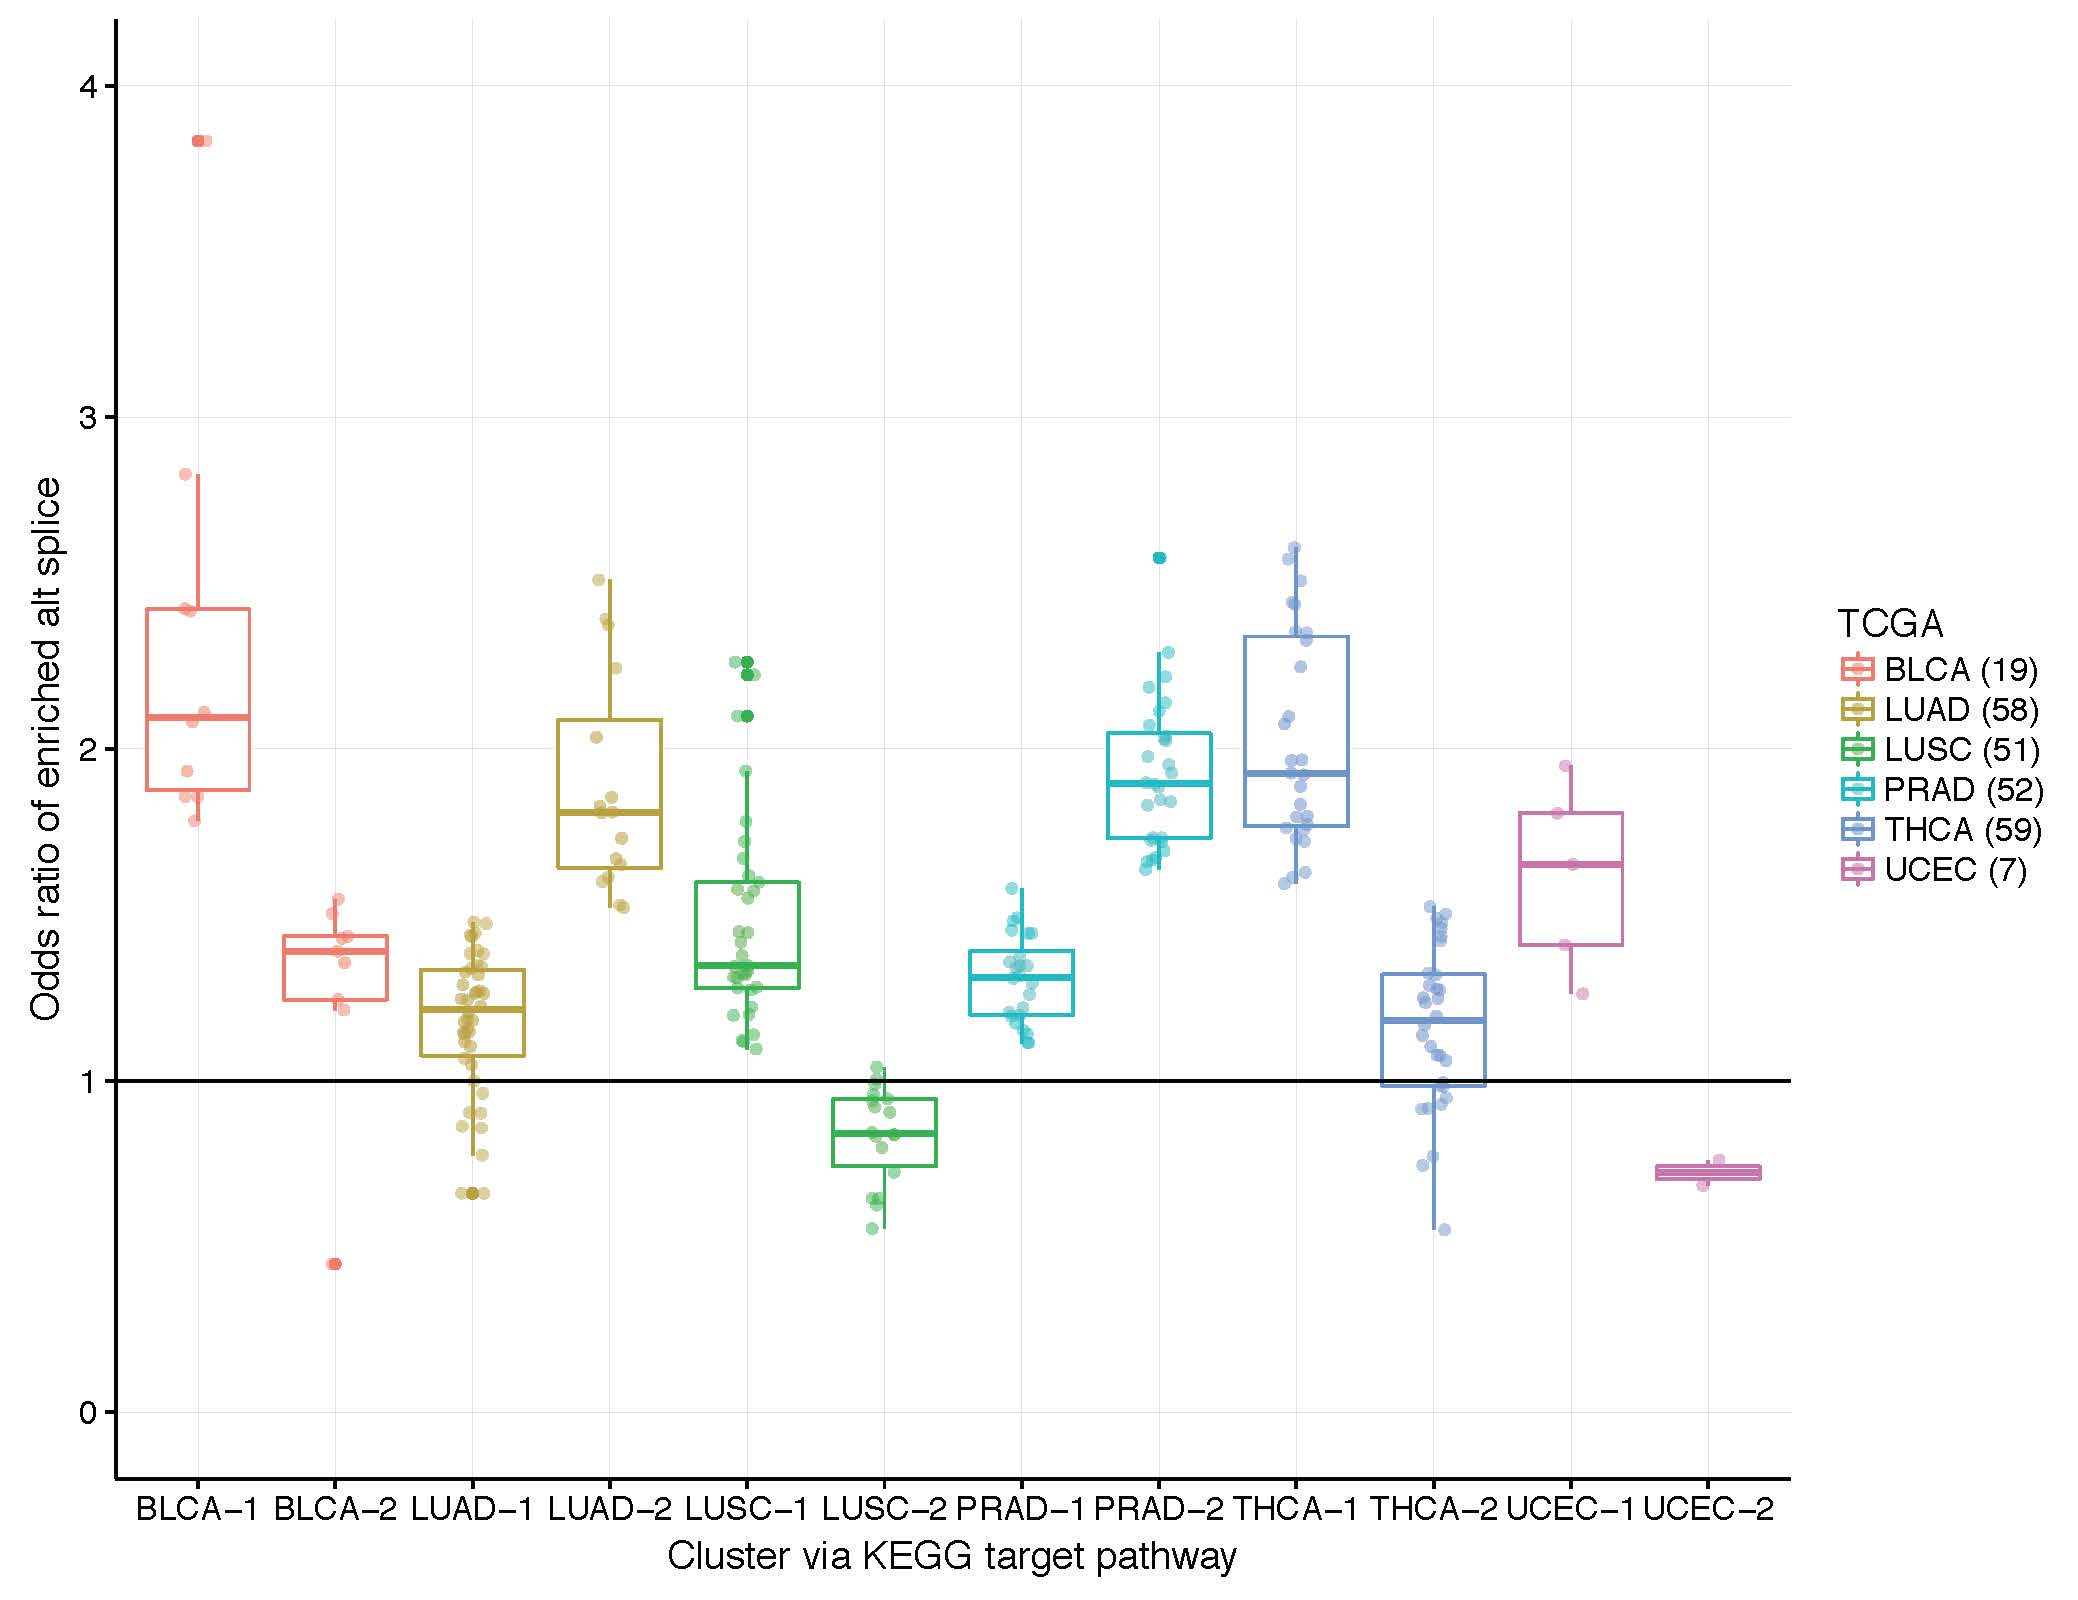
\includegraphics[keepaspectratio,width=\textwidth,height=0.8\textheight]{../n1pas/figures/Figure3.jpg}
\end{figure}

\end{frame}

\begin{frame}{%
\protect\hypertarget{survival-subtyping-pipeline-using-n1pas}{%
Survival subtyping pipeline using N1PAS}}

\begin{figure}[htb]
  \centering 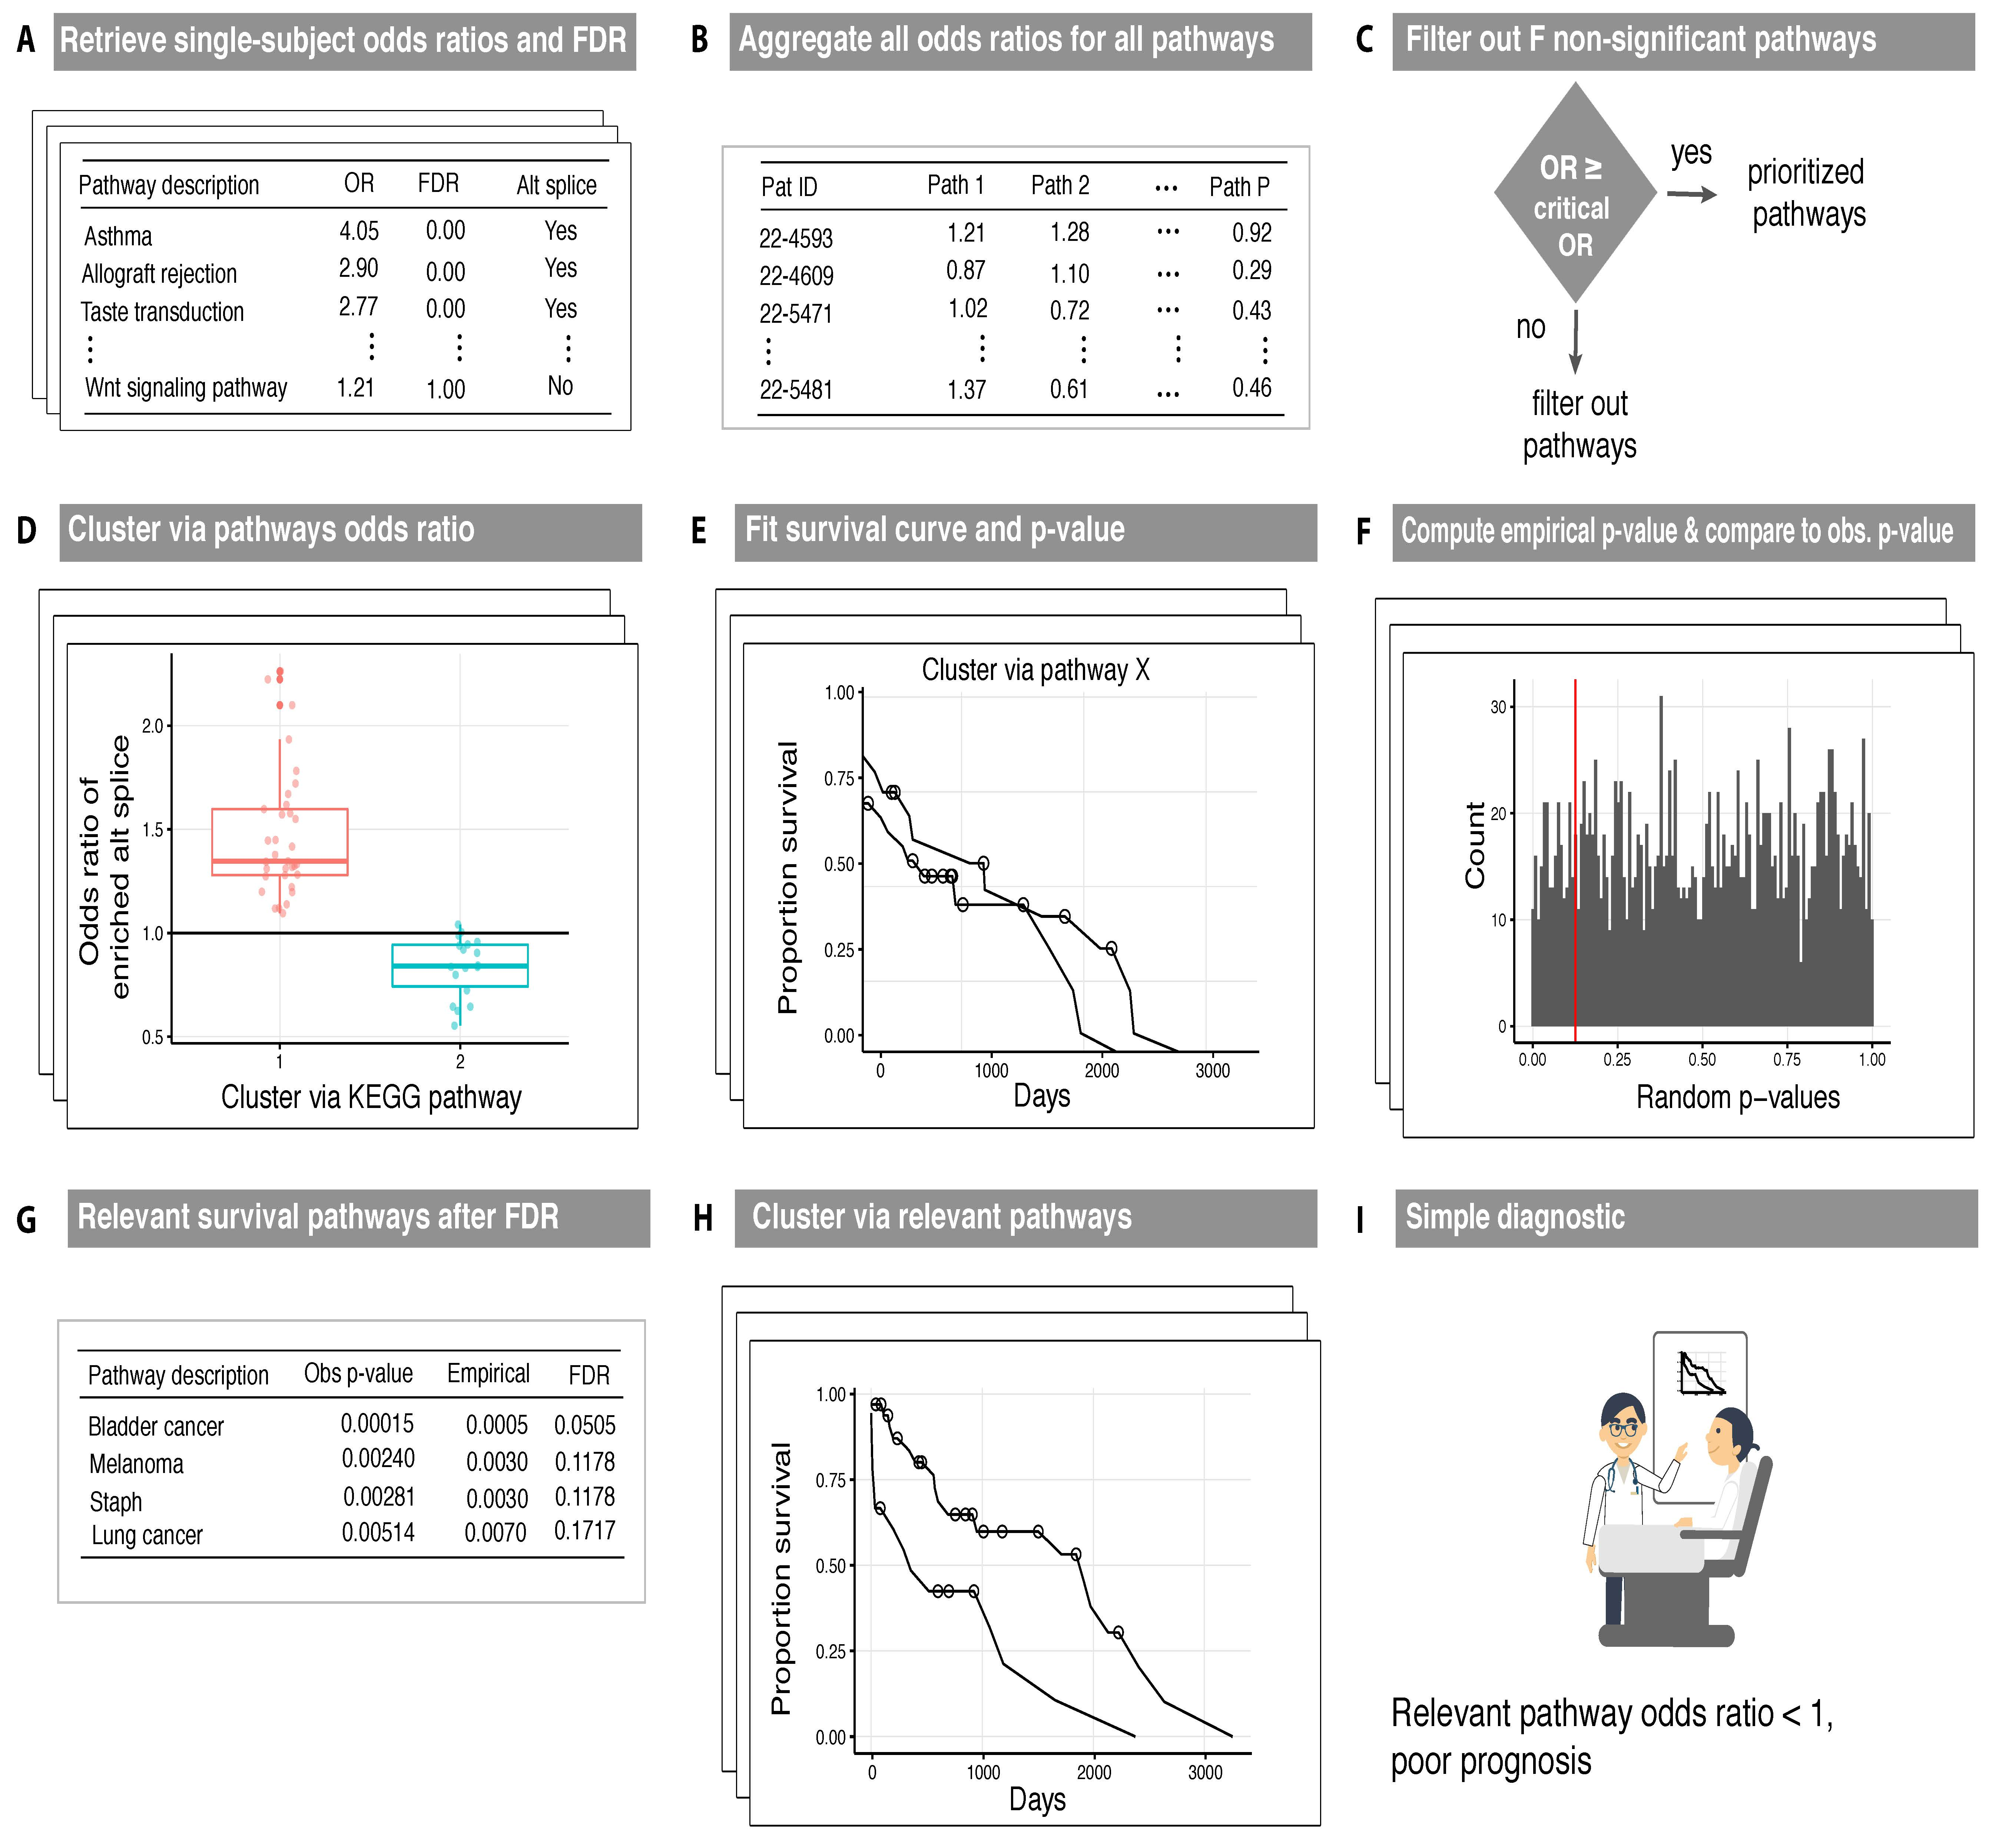
\includegraphics[keepaspectratio,width=\textwidth,height=0.8\textheight]{../n1pas/figures/Figure2.jpg}
\end{figure}

\end{frame}

\begin{frame}{%
\protect\hypertarget{non-small-cell-lung-cancer-lusc-pathways-selected-by-subtyping-pipeline}{%
Non-small cell lung cancer (LUSC) pathways selected by subtyping
pipeline}}

\begin{figure}[htb]
  \centering 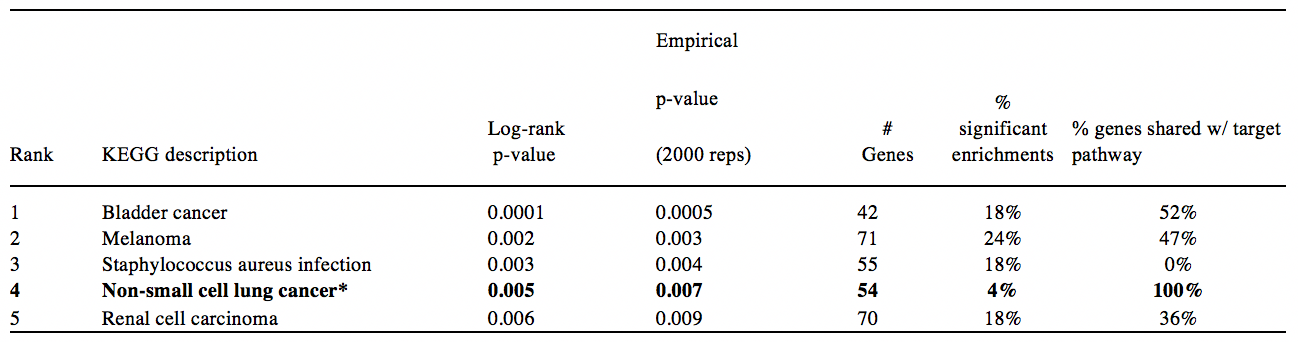
\includegraphics[keepaspectratio,width=\textwidth,height=0.8\textheight]{../n1pas/figures/table3.png}
\end{figure}

\end{frame}

\begin{frame}{%
\protect\hypertarget{summary}{%
Summary}}

\begin{enumerate}
  \item We developed the N-of-1-pathways Alternatively Spliced (N1PAS) framework.
    \item This will provide a single-subject method to detect alternatively spliced genetic pathways to enable precision medicine.
    \item We conducted Monte Carlo evaluations and find adequate false discovery rate control and impressive power to detect enriched pathways.
    \item We validated the method using target KEGG pathways.
    \item And applied N1PAS output to survival subtyping.
    \item Implemented an R package \url{https://github.com/grizant/n1pas/tree/master}.
  \end{enumerate}

\end{frame}

\begin{frame}{%
\protect\hypertarget{project-2-learning-therapeutic-resistance-from-circulating-tumor-cells-ctcs}{%
Project 2 Learning therapeutic resistance from circulating tumor cells
(CTCs)}}

\begin{itemize}
\tightlist
\item
  Can prostate cancer therapy resistance be detected from single cell
  RNA-sequencing (scRNA-eq) of CTCs?
\item
  But it is experimentally and computational challenging to sequence
  CTCs.
\item
  This results in only a few CTCs sequenced per patient.
\item
  You need a tailored (bespoke) method to handle this question.
\item
  This lead to the development of an \emph{Analysis of aggregated
  cell-cell statistical distances within pathways unveils
  therapeutic-resistance mechanisms in circulating tumor cells}
  Schissler et al. (2016)
\end{itemize}

\end{frame}

\begin{frame}{%
\protect\hypertarget{ctcs-1}{%
CTCs 1}}

\begin{figure}[htb]
  \centering \includegraphics[keepaspectratio,width=\textwidth,height=0.8\textheight]{../CTCs/figures/fig1.pdf}
\end{figure}

\end{frame}

\begin{frame}{%
\protect\hypertarget{ctcs-2}{%
CTCs 2}}

\begin{figure}[htb]
  \centering \includegraphics[keepaspectratio,width=\textwidth,height=0.8\textheight]{../CTCs/figures/fig3.pdf}
\end{figure}

\end{frame}

\begin{frame}{%
\protect\hypertarget{ctcs-3}{%
CTCs 3}}

\begin{figure}[htb]
  \centering \includegraphics[keepaspectratio,width=\textwidth,height=0.8\textheight]{../CTCs/figures/fig4.pdf}
\end{figure}

\end{frame}

\begin{frame}{%
\protect\hypertarget{ctcs-4}{%
CTCs 4}}

\begin{figure}[htb]
  \centering \includegraphics[keepaspectratio,width=\textwidth,height=0.8\textheight]{../CTCs/figures/fig5.pdf}
\end{figure}

\end{frame}

\begin{frame}{%
\protect\hypertarget{conclusions-future-work-learn-more}{%
Conclusions / Future Work / Learn more}}

\begin{itemize}
\tightlist
\item
  explore the role of subjective (informative) prior distribution
  ellicitation in Bayesian bioinformatic modeling.
\item
  Students consider taking the new STAT 646 Introduction to Bayesian
  Statistics. I’ll do a project with you and I encourage you to bring
  your thesis research. Faculty also sit in
\end{itemize}

\end{frame}

\begin{frame}{%
\protect\hypertarget{acknowledgements}{%
Acknowledgements}}

\begin{columns}[T]
  \begin{column}{0.55\columnwidth}
    \begin{block}{Math \& Stats, University of Nevada, Reno}
      Alex Knudson, MS Stat student\\
      Anna Panorska, PhD\\
      Tomasz Kozubowski, PhD
    \end{block}
    \begin{block}{University of Arizona}
      Walter W.~Piegorsch, PhD\\
      Edward J.~Bedrick, PhD
      D.~Dean Billheimer, PhD\\
      Hao Helen Zhang, PhD\\
      Qike Li, PhD\\
      Ikbel Achour, PhD\\
      Joanne Berghout, PhD
    \end{block}
  \end{column}

\begin{column}{0.45\columnwidth}
    \begin{block}{Medical doctors}
      Yves A.~Lussier, MD
    \end{block}
    %\begin{block}{Grants/travel awards}
    %  Research \& Innovation, UNR
    % \end{block}
    \begin{block}{Biochemistry, UNR}
      Thanks Dr. Ian Wallace for the invitation\\
      Colin Fox, PhD candidate\\
      All others involved
    \end{block}
  \end{column}
\end{columns}

\end{frame}

\begin{frame}{%
\protect\hypertarget{references}{%
6.2 References}}

\hypertarget{refs}{}
\leavevmode\hypertarget{ref-Efron2007a}{}%
Efron, Bradley. 2007. “Correlation and large-scale simultaneous
significance testing.” \emph{Journal of the American Statistical
Association} 102 (477):93–103.
\url{https://doi.org/10.1198/016214506000001211}.

\leavevmode\hypertarget{ref-Efron2013}{}%
———. 2013. “Local False Discovery Rates.” In \emph{Large-Scale
Inference}. \url{https://doi.org/10.1017/cbo9780511761362.006}.

\leavevmode\hypertarget{ref-Graveley2001}{}%
Graveley, Brenton R. 2001. “Alternative splicing: Increasing diversity
in the proteomic world.”
\url{https://doi.org/10.1016/S0168-9525(00)02176-4}.

\leavevmode\hypertarget{ref-Johnson2017}{}%
Johnson, Marla, and Elizabeth Purdom. 2017. “Clustering of mRNA-Seq data
for detection of alternative splicing patterns.” \emph{Biostatistics} 18
(2):295–307. \url{https://doi.org/10.1101/021733}.

\leavevmode\hypertarget{ref-kanehisa2000kegg}{}%
Kanehisa, Minoru, and Susumu Goto. 2000. “KEGG: kyoto encyclopedia of
genes and genomes.” \emph{Nucleic Acids Research} 28 (1). Oxford Univ
Press:27–30.

\leavevmode\hypertarget{ref-Khatri2012n1pas}{}%
Khatri, Purvesh, Marina Sirota, and Atul J. Butte. 2012. “Ten years of
pathway analysis: Current approaches and outstanding challenges.”
\url{https://doi.org/10.1371/journal.pcbi.1002375}.

\leavevmode\hypertarget{ref-Schissler2016a}{}%
Schissler, A.G., Q. Li, J.L. Chen, C. Kenost, I. Achour, D.D.
Billheimer, H. Li, W.W. Piegorsch, and Y.A. Lussier. 2016. “Analysis of
aggregated cell-cell statistical distances within pathways unveils
therapeutic-resistance mechanisms in circulating tumor cells.”
\emph{Bioinformatics} 32 (12).
\url{https://doi.org/10.1093/bioinformatics/btw248}.

\leavevmode\hypertarget{ref-Subramanian2005}{}%
Subramanian, A., P. Tamayo, V. K. Mootha, S. Mukherjee, B. L. Ebert,
Michael A Gillette, A. Paulovich, et al. 2005. “Gene set enrichment
analysis: A knowledge-based approach for interpreting genome-wide
expression profiles.” \emph{Proceedings of the National Academy of
Sciences}. \url{https://doi.org/10.1073/pnas.0506580102}.

\end{frame}

\end{document}
